\chapter{Force magnétique}

\paragraph{Objectif}

\begin{enumerate}
  \item L'étudiant connaîtra l'expression de la force magnétique sur une
    particule chargée.
  \item L'étudiant pourra analyser un mouvement circulaire.
  \item L'étudiant comprendra le fonctionnement du sélecteur de vitesse, du
    spectromètre de masse.
\end{enumerate}



\section{Force magnétique sur une charge ponctuelle}

\marginnote{
  Lafrance \S 9.1, 9.2

  Tremblay \S 8.3, 8.4
}

\begin{fondamentalbox}
La force magnétique est proportionnelle à la charge, à la vitesse et au champ
magnétique. De plus, elle est perpendiculaire à la fois au champ magnétique et
à la vitesse.
$$\vF = q \vv \times \vB$$
\end{fondamentalbox}


\begin{diapobox}
  \marginnote{
    \begin{center}
      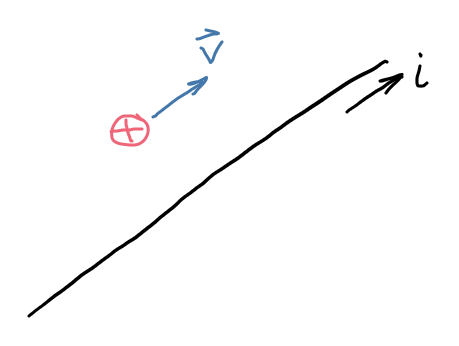
\includegraphics[scale=0.3]{09-force-magnetique/figures/proton_fil.png}
    \end{center}
  }
  Un proton a une vitesse parallèle à un long fil parcouru d'un courant $i$. La
  vitesse du proton est dans la même direction que le courant.
  Le proton 
  \begin{enumerate}
    \item se rapprochera du fil
    \item s'éloignera du fil
    \item continuera son chemin en ligne droite
  \end{enumerate}
\end{diapobox}

\begin{diapobox}
  \marginnote{
    \begin{center}
      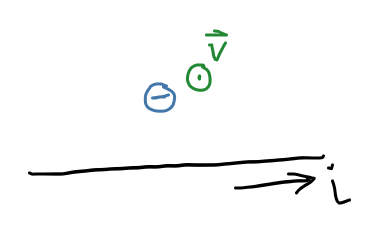
\includegraphics[scale=0.3]{09-force-magnetique/figures/electron_fil.png}
    \end{center}
  }
  Un électron a une vitesse perpendiculaire à un long fil parcouru d'un courant
  $i$. La force sur l'électron est 
  \begin{enumerate}
    \item vers le fil
    \item parallèle au fil
    \item nulle
    \item pointe en s'éloignant du fil
  \end{enumerate}
\end{diapobox}



\subsection*{Exemple - Mouvement circulaire}

On envoie des particules avec une vitesse horizontale de \SI{3.52e5}{m/s} dans
une région où existe un champ magnétique uniforme de \SI{1}{G} vers le bas. On
observe qu'à leur arrivée dans le champ magnétique, les particules tournent
dans le sens horaire lorsqu'on les regarde du dessus. Le rayon de leur
trajectoire est de \SI{2}{cm}.

\begin{enumerate}
  \item Déterminer le signe de la charge de ces particules.
  \item Déterminer le rapport $q/m$ pour ces particules.
  \item Déterminer la fréquence de leur mouvement.
\end{enumerate}


Signe est négatif car $\vv \times \vB$ pointe dans le sens anti-horaire donc la
charge doit être négative.

La force qui agit sur ces particules est
\begin{align*}
  \vF &= q\vv \times \vB \\
  F &= \abs{q} vB
\end{align*}
Par la deuxième loi de Newton,
\begin{align*}
  F &= \frac{mv^2}{R} \\ 
    &= \abs{q} vB
\end{align*}
Donc
\begin{align*}
  \frac{\abs{q}}{m} &= \frac{v}{RB} \\
  &= \SI{1.76e11}{C/kg}
\end{align*}

(Ce sont des électrons!)

Pour déterminer la fréquence, on veut savoir combien de tours sont effectués
chaque seconde.
\begin{align*}
  f &= \frac{v}{2\pi R} \\
    &= \SI{2.80e6}{Hz} = \SI{2.80}{MHz}
\end{align*}


\subsection*{Force de Lorentz}

Si une particule chargée est dans une région où il y a à la fois un champ
magnétique et un champ électrique, alors la force totale sur la particule est
la somme de la force électrique et de la force magnétique
$$\vF = q\vv \times \vB + q \vE$$



\subsection*{Exemple - Sélecteur de vitesse}

Des particules $\alpha$ sont envoyées dans une région où se trouvent un champ
électrique uniforme de \SI{236}{V/m} et un champ magnétique uniforme
perpendiculaire de \SI{155}{mT}. Quelle est l'énergie cinétique des particules
$\alpha$ qui continuent leur trajectoire en ligne droite?


La force est
\begin{align*}
  \vF &= q(\vv \times \vB + \vE) \\
      &= 0 \\
  \vv \times \vB &= -\vE \\
  v &= \frac{E}{B \sin \theta} \\
  v &= \SI{1522.58}{m/s} \\
  K &= \frac{1}{2} \times \SI{6.6465e-27}{kg} (\SI{1522.58}{m/s})^2 \\
    &= \SI{48.1}{meV}
\end{align*}


%\subsection*{Exemple - Spectromètre de masse}

%On considère un spectromètre de masse avec un champ magnétique de \SI{10}{G}.
%On envoie des ions +1 de nickel 58 (\SI{57.935}{u}) et de nickel 60
%(\SI{59.931}{u}).  Un sélecteur de vitesse s'assure que la vitesse de tous les
%ions est de \SI{1e5}{m/s}. Quelle est la distance entre les points où arrivent
%les deux isotopes de nickel?


%\begin{align*}
  %\frac{mv^2}{R} &= \abs{q} vB \\
  %R &= \frac{mv^2}{qvB} \\
  %D &= 2R_2 - 2R_1 \\
   %&= 2(m_2 - m_1) \frac{v}{qB} \\
   %&= \SI{0.414}{mm}
%\end{align*}


\section{Force magnétique sur les fils}

\marginnote{
  Lafrance \S 9.5
}

Si on a un fil parcouru d'un courant dans un champ magnétique, le fil subira
une force. En effet, les électrons se déplacent parce qu'il y a un courant.
Leur vitesse est la vitesse de dérive donc la force sur les charges mobiles est
\begin{align*}
  \vF_1 = q\vv \times \vB
\end{align*}
et la force totale est la somme de toutes les forces sur les porteurs de
charge soit
\begin{align*}
  \vF &= \sum \vF_1  \\
      &= \sum q \vv \times \vB
\end{align*}
Toutes les charges se déplacent à la même vitesse et se trouvent dans le même
champ magnétique donc on peut mettre en évidence le produit vectoriel
\begin{align*}
  \vF &= \left( \sum q \right) \vv \times \vB
\end{align*}
La quantité entre parenthèse est la charge totale qui se déplace qu'on peut
aussi écrire comme le produit du volume du fil $A\ell$, de la densité
volumique de charge $n$ et de la charge d'un porteur de charge
\begin{align*}
  \vF &= nA\ell q \vv \times \vB
\end{align*}
On se rappelle que le courant est définit comme $i = nAqv$ donc, en définissant
le vecteur $\vec{\ell}$ comme un vecteur de longueur $\ell$ qui pointe dans la
direction du courant,
\begin{align*}
  \vF = i\vec{\ell} \times \vB
\end{align*}

\begin{diapobox}
  \marginnote{
    \begin{center}
      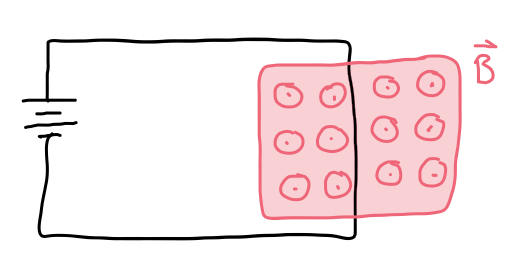
\includegraphics[width=3cm]{09-force-magnetique/figures/fil_dans_mag.png}
    \end{center}
  }
  Une section de fil de \SI{8}{\centi\meter} parcouru d'un courant de
  \SI{10}{\ampere} se trouve dans un champ magnétique uniforme de
  \SI{5}{\tesla}. Quelle est la force sur le fil?
\end{diapobox}

\begin{reponsebox}
  La force est vers la gauche (RMD) et de grandeur
  \begin{align*}
    F &= ilB \sin\SI{90}{\degree}  \\
      &= ilB  \\
      &= \SI{4}{\newton}
  \end{align*}
\end{reponsebox}


\begin{diapobox}
  \marginnote{
    \begin{center}
      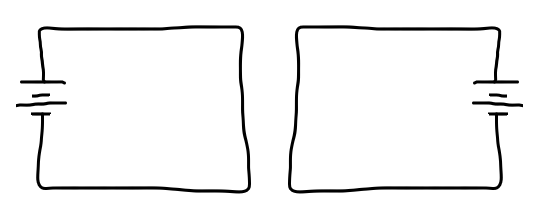
\includegraphics[width=3cm]{09-force-magnetique/figures/deux_fils.png}
    \end{center}
  }
  Une section de fil de \SI{8}{\centi\meter} parcouru d'un courant de
  \SI{10}{\ampere} se trouve à proximité d'une section de fil parallèle de même
  longueur parcouru d'un courant de \SI{5}{\ampere}. Les deux fils sont séparés
  d'une distance de \SI{2}{\centi\meter}.
  \begin{enumerate}
    \item Quelle est la force sur le fil de gauche?
    \item Quelle est la force sur le fil de droite?
  \end{enumerate}

\end{diapobox}

\begin{reponsebox}
  La force est vers la droite (RMD) et de grandeur
  \begin{align*}
    F &= i_1lB_2 \sin\SI{90}{\degree}  \\
      &= i_1lB_2  \\
      &= i_1 l \frac{\mu_0 i_2}{2\pi r}  \\
      &= \SI{4e-5}{\newton}
  \end{align*}
  La force sur le fil de droite est de même grandeur et vers la gauche, par la
  troisième loi de Newton.
\end{reponsebox}


\subsection{Moteur simple}

\marginnote{
  Lafrance \S 9.6
}

Un moteur est simplement une boucle (ou une bobine) de fil qui se trouve dans
un champ magnétique (produit par un aimant permanent ou un électroaimant). Le
fil est parcouru d'un courant dont la direction est changée à chaque demi-tour
grâce à un petit tour de passe passe mécanique qu'on appelle un commutateur.
L'idée est d'exercer un moment de force sur la boucle grâce au champ
magnétique.

\begin{diapobox}
  \marginnote{
    \begin{center}
      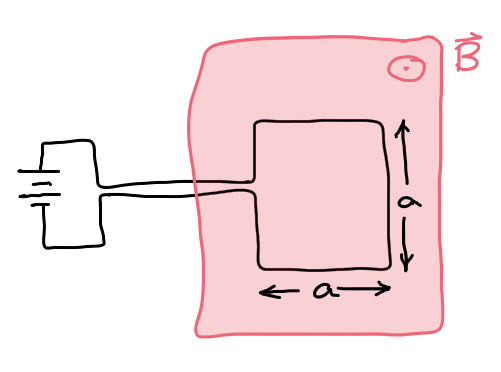
\includegraphics[width=3cm]{09-force-magnetique/figures/boucle_dans_mag.png}
    \end{center}
  }
  Déterminer la force magnétique sur la boucle suivante.

  \begin{enumerate}
    \item $iaB$
    \item $4iaB$
    \item $ia^2B$
    \item $0$
  \end{enumerate}

  Est-ce que la boucle tournera?

  \begin{enumerate}
    \item Oui, la partie du haut s'approchera de nous
    \item Oui, la partie du haut s'éloignera de nous
    \item Oui, la partie de droite s'approchera de nous
    \item Non
  \end{enumerate}
\end{diapobox}

\begin{diapobox}
  \marginnote{
    \begin{center}
      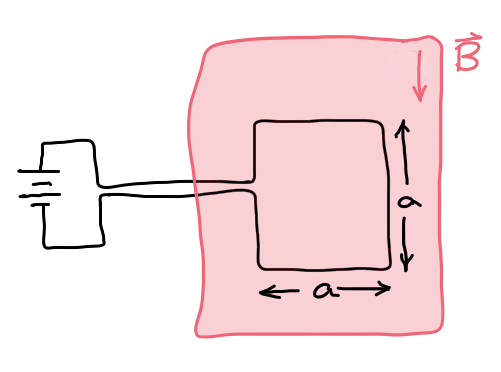
\includegraphics[width=3cm]{09-force-magnetique/figures/boucle_dans_mag_2.png}
    \end{center}
  }
  Déterminer la force magnétique sur la boucle suivante.

  \begin{enumerate}
    \item $iaB$
    \item $4iaB$
    \item $ia^2B$
    \item $0$
  \end{enumerate}

  Est-ce que la boucle tournera?

  \begin{enumerate}
    \item Oui, la partie du haut s'approchera de nous
    \item Oui, la partie du haut s'éloignera de nous
    \item Oui, la partie de droite s'approchera de nous
    \item Non
  \end{enumerate}
\end{diapobox}
